\newpage
\section{Lecture-04}
\subsection{Scalar Functions of Several Variables}

In many areas of mathematics, we encounter quantities that depend on more than one variable. For instance, the temperature in a room may depend on position, the elevation of a landscape depends on location, and the pressure of a gas may depend on both volume and temperature. These are all examples of \emph{scalar functions of several variables}: functions that assign a real number to each point in $\mathbb{R}^n$.

\begin{definition}
A \emph{scalar function of several variables} is a function
\[
f:\mathbb{R}^n\to\mathbb{R}.
\]
Thus, to each point
\[
\vec x=
\begin{pmatrix}
x_1\\
\vdots\\
x_n
\end{pmatrix}
\in\mathbb{R}^n,
\]
the function assigns a real number $f(\vec x)$.

In practice, instead of writing
\[
f\left(
\begin{pmatrix}
x_1\\
\vdots\\
x_n
\end{pmatrix}
\right),
\]
it is more convenient to write simply
\[
f(x_1,\dots,x_n) \text{ or } f\begin{pmatrix}
x_1\\
\vdots\\
x_n
\end{pmatrix}.
\]
This is only a change in notation; the meaning is the same.
\end{definition}

\begin{definition}
Let $f:\mathbb{R}^n\to\mathbb{R}$. The \emph{graph} of $f$ is the subset of $\mathbb{R}^{n+1}$ defined by
\[
\operatorname{graph}(f)
=
\left\{
\begin{pmatrix}
\vec x\\
f(\vec x)
\end{pmatrix}
: \vec x\in\mathbb{R}^n
\right\}.
\]
Equivalently, the graph is the set of all points $(x_1,\dots,x_n,f(x_1,\dots,x_n))$ in $\mathbb{R}^{n+1}$.
\end{definition}

When $n=1$ or $n=2$, the graph often gives a useful geometric picture of the function. For functions of two variables, one may think of the graph as a surface in $\mathbb{R}^3$.

Another helpful way to visualize a function is through its \emph{level sets}. For a constant $c\in\mathbb{R}$, the level set of $f$ corresponding to $c$ is the set
\[
\{\vec x\in\mathbb{R}^n : f(\vec x)=c\}.
\]
In the case $n=2$, these are often called \emph{level curves} or \emph{contour curves}, since they resemble the contour lines on a topographic map.

\begin{example}
    Let $f:\mathbb{R}^2\to\mathbb{R}$ be defined by
    \[
     f(x,y)=\sqrt{1-\frac{x^2}{9}-\frac{y^2}{4}}
    \]
    Find the domain and range of $f$, and describe its graph and level curves for various values of $c=0,1$.
\end{example}

\begin{example}
Define $f:\mathbb{R}^2\to\mathbb{R}$ by
\[
f(x,y)=x^2+y^2.
\]
Then $f$ assigns to each point $(x,y)$ the square of its distance from the origin.

Its graph is the set
\[
\operatorname{graph}(f)
=
\{(x,y,x^2+y^2): (x,y)\in\mathbb{R}^2\},
\]
which is a paraboloid in $\mathbb{R}^3$.

For each constant $c\ge 0$, the level curve $f(x,y)=c$ is given by
\[
x^2+y^2=c,
\]
which is a circle centered at the origin with radius $\sqrt{c}$.
\begin{center}
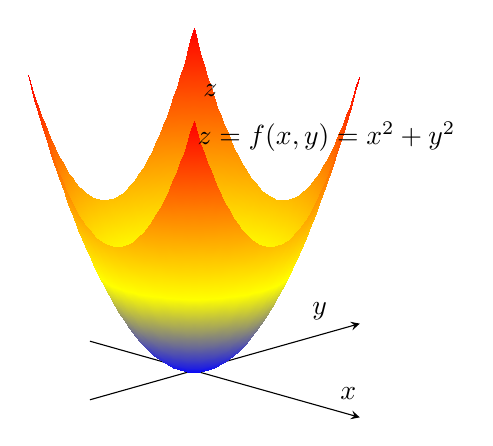
\begin{tikzpicture}
\begin{axis}[
    axis lines=middle,
    xlabel={$x$},
    ylabel={$y$},
    zlabel={$z$},
    xtick=\empty,
    ytick=\empty,
    ztick=\empty,
    domain=-2:2,
    y domain=-2:2,
    samples=50,
    samples y=50,
    view={45}{20},
    xmin=-2.5, xmax=4,
    ymin=-2.5, ymax=4,
    zmin=0, zmax=8,
]
\addplot3[
    surf,
    shader=interp,
]
{x^2+y^2};

\node at (axis cs:1.4,1.8,6.2) {$z=f(x,y)=x^2+y^2$};
\end{axis}
\end{tikzpicture}
\end{center}
\end{example}
\subsection{Vector Functions of Several Variables}

In many mathematical settings, the quantity we wish to study is not a single real number but a vector. For example, the velocity of a moving particle has several components, a force field assigns a vector to each point in space, and a parametrized curve records position as a vector depending on one or more variables. This leads naturally to the notion of a \emph{vector-valued function of several variables}.

Such functions take points in $\mathbb{R}^n$ as inputs and return vectors in $\mathbb{R}^m$. In practice, they may be viewed either as geometric mappings or as collections of scalar component functions. Both points of view are useful, and we will move freely between them.

\begin{definition}
A \emph{vector function of several variables} is a function
\[
\mathbf{f}:\mathbb{R}^n\to\mathbb{R}^m.
\]
Thus, for each point
\[
\vec x=
\begin{pmatrix}
x_1\\
\vdots\\
x_n
\end{pmatrix}
\in\mathbb{R}^n,
\]
the value $\mathbf{f}(\vec x)$ is a vector in $\mathbb{R}^m$.

If
\[
\mathbf{f}(\vec x)=
\begin{pmatrix}
f_1(\vec x)\\
\vdots\\
f_m(\vec x)
\end{pmatrix},
\]
then each $f_i:\mathbb{R}^n\to\mathbb{R}$ is a scalar-valued function, called the $i$th \emph{component function} of $\mathbf{f}$. In this way, a vector-valued function may be regarded as a collection of $m$ scalar-valued functions of $n$ variables.
\end{definition}

It is often convenient to write the input vector in coordinate form. Thus, instead of writing $\mathbf{f}(\vec x)$, where
\[
\vec x=
\begin{pmatrix}
x_1\\
\vdots\\
x_n
\end{pmatrix},
\]
we may simply write
\[
\mathbf{f}(x_1,\dots,x_n).
\]
This is only a notational simplification.

\begin{definition}
Let $\mathbf{f}:\mathbb{R}^n\to\mathbb{R}^m$ be a vector-valued function. If
\[
\mathbf{f}(\vec x)=
\begin{pmatrix}
f_1(\vec x)\\
\vdots\\
f_m(\vec x)
\end{pmatrix},
\]
then $\mathbf{f}$ is said to be determined by its component functions
\[
f_1,\dots,f_m:\mathbb{R}^n\to\mathbb{R}.
\]
Accordingly, many properties of $\mathbf{f}$ can be studied by examining its components one at a time.
\end{definition}

Vector-valued functions are especially important in geometry and applied mathematics. They arise in the study of parametrized curves and surfaces, as well as in vector fields such as velocity fields, gravitational fields, and electromagnetic fields.

\begin{example}
Define $\mathbf{f}:\mathbb{R}^2\to\mathbb{R}^3$ by
\[
\mathbf{f}(u,v)=
\begin{pmatrix}
u\\
v\\
u^2+v^2
\end{pmatrix}.
\]
Then $\mathbf{f}$ is a vector-valued function of two variables.

Its component functions are
\[
f_1(u,v)=u,\qquad f_2(u,v)=v,\qquad f_3(u,v)=u^2+v^2.
\]
Geometrically, $\mathbf{f}$ assigns to each point $(u,v)$ in the plane the point
\[
(u,v,u^2+v^2)
\]
in $\mathbb{R}^3$. Thus, $\mathbf{f}$ parametrizes the paraboloid
\[
z=x^2+y^2.
\]
\end{example}

\begin{example}
Define $\mathbf{F}:\mathbb{R}^2\to\mathbb{R}^2$ by
\[
\mathbf{F}(x,y)=
\begin{pmatrix}
-y\\
x
\end{pmatrix}.
\]
This is a vector field in the plane. At each point $(x,y)$, the function assigns the vector $(-y,x)$.

Its component functions are
\[
F_1(x,y)=-y,\qquad F_2(x,y)=x.
\]
This field represents a rotational pattern about the origin, since each vector is perpendicular to the position vector $(x,y)$.
\end{example}
~\\
For more interactive visualizations of scalar and vector functions, see \url{https://mathinsight.org/level_sets}.

\subsection{Limits of Functions of One Variable}
\begin{definition}
Let $I$ be an open interval containing $c$, and let $f$ be a function defined on $I$, except possibly at $c$. We say that the \emph{limit} of $f(x)$ as $x$ approaches $c$ is $L$, and write
\[
\lim_{x\to c} f(x)=L,
\]
if for every $\varepsilon>0$, there exists $\delta>0$ such that for all $x\neq c$, 
\[
|x-c|<\delta \implies |f(x)-L|<\varepsilon.
\]
\end{definition}
\begin{example}
Show that
\[
\lim_{x\to 4}\sqrt{x}=2.
\]

\bigskip
\noindent\textbf{Solution:}

Before we use the formal definition, let us first try some numerical tolerances.
Suppose the $y$-tolerance is $0.5$, or $\varepsilon=0.5$.
How close to $4$ does $x$ have to be so that $y$ is within $0.5$ units of $2$,
that is, so that $1.5<y<2.5$?
Since $y=\sqrt{x}$, we proceed as follows:
\[
1.5<y<2.5
\]
\[
1.5<\sqrt{x}<2.5
\]
\[
1.5^2<x<2.5^2
\]
\[
2.25<x<6.25.
\]

So, what is the desired $x$-tolerance?
We want a symmetric interval of $x$-values, namely
\[
4-\delta < x < 4+\delta.
\]
The lower bound $2.25$ is $1.75$ units from $4$, while the upper bound $6.25$ is
$2.25$ units from $4$.
We need the smaller of these two distances, so we must have
\[
\delta \le 1.75.
\]

\bigskip

\begin{center}
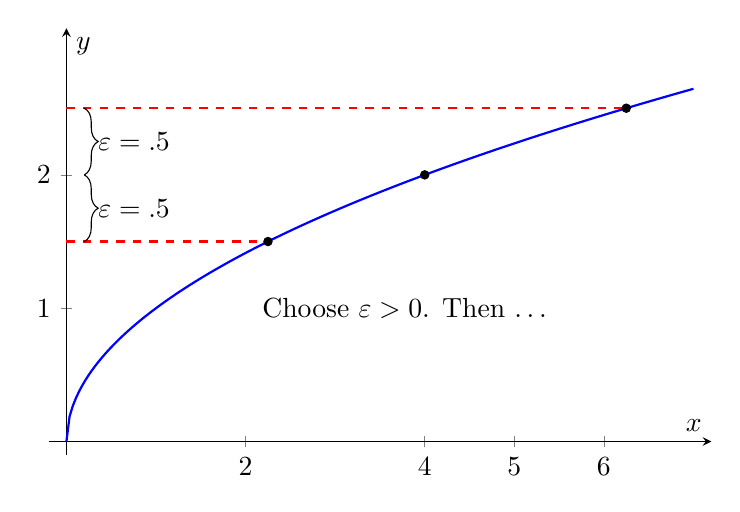
\begin{tikzpicture}
\begin{axis}[
    width=10cm,
    height=7cm,
    axis lines=middle,
    xmin=-0.2, xmax=7.2,
    ymin=-0.1, ymax=3.1,
    xtick={2,4,5,6},
    ytick={1,2},
    xlabel={$x$},
    ylabel={$y$},
    domain=0:7,
    samples=200,
    clip=false
]

% Curve y = sqrt(x)
\addplot[blue, thick] {sqrt(x)};

% Points
\addplot[only marks, mark=*, mark size=1.5pt] coordinates {(2.25,1.5) (4,2) (6.25,2.5)};

% Dashed epsilon lines
\addplot[red, dashed, thick] coordinates {(0,1.5) (2.25,1.5)};
\addplot[red, dashed, thick] coordinates {(0,2.5) (6.25,2.5)};

% Braces for epsilon
\draw[decorate,decoration={brace,mirror,amplitude=5pt}]
    (axis cs:0.2,1.5) -- (axis cs:0.2,2)
    node[midway,xshift=18pt] {$\varepsilon=.5$};

\draw[decorate,decoration={brace,mirror,amplitude=5pt}]
    (axis cs:0.2,2) -- (axis cs:0.2,2.5)
    node[midway,xshift=18pt] {$\varepsilon=.5$};

% Label in plot
\node at (axis cs:3.8,1.0) {Choose $\varepsilon>0$. Then \dots};

\end{axis}
\end{tikzpicture}
\end{center}

\begin{center}
\begin{tikzpicture}
\begin{axis}[
    width=9cm,
    height=6.8cm,
    axis lines=middle,
    xmin=-0.2, xmax=7.0,
    ymin=-0.1, ymax=3.1,
    xtick={2,4,6},
    ytick={1,2},
    xlabel={$x$},
    ylabel={$y$},
    domain=0:6.8,
    samples=200,
    clip=false
]

% curve
\addplot[blue, thick] {sqrt(x)};

% key points
\addplot[only marks, mark=*, mark size=1.3pt]
coordinates {(2.25,1.5) (4,2) (6.25,2.5)};

% dashed horizontal epsilon lines
\addplot[gray, dashed] coordinates {(0,1.5) (2.25,1.5)};
\addplot[gray, dashed] coordinates {(0,2.5) (6.25,2.5)};

% dashed vertical red lines
\addplot[red, dashed] coordinates {(2.25,0) (2.25,1.5)};
\addplot[red, dashed] coordinates {(6.25,0) (6.25,2.5)};

% epsilon braces
\draw[decorate,decoration={brace,mirror,amplitude=5pt}]
(axis cs:0.22,1.5) -- (axis cs:0.22,2)
node[midway,xshift=18pt] {$\varepsilon=.5$};

\draw[decorate,decoration={brace,mirror,amplitude=5pt}]
(axis cs:0.22,2) -- (axis cs:0.22,2.5)
node[midway,xshift=18pt] {$\varepsilon=.5$};

% bottom braces for widths
\draw[decorate,decoration={brace,mirror,amplitude=4pt}]
(axis cs:2.25,0.25) -- (axis cs:4,0.25)
node[midway,yshift=-12pt] {\scriptsize width};

\node at (axis cs:3.12,0.47) {\scriptsize $=1.75$};

\draw[decorate,decoration={brace,mirror,amplitude=4pt}]
(axis cs:4,0.25) -- (axis cs:6.25,0.25)
node[midway,yshift=-12pt] {\scriptsize width};

\node at (axis cs:5.12,0.47) {\scriptsize $=2.25$};

% explanatory labels
\node at (axis cs:4.35,1.52) {$\cdots\ \text{choose }\delta\text{ smaller}$};
\node at (axis cs:4.25,1.18) {$\text{than each of these}$};

% small arrows
\draw[-{Stealth[length=2mm]}, thin] (axis cs:4.15,1.03) -- (axis cs:3.0,0.82);
\draw[-{Stealth[length=2mm]}, thin] (axis cs:4.35,1.03) -- (axis cs:5.25,0.82);

\end{axis}
\end{tikzpicture}

\vspace{0.4em}
{\large With $\varepsilon=0.5$, we pick any $\delta<1.75$.}
\end{center}

\bigskip

Given the $y$ tolerance $\varepsilon=0.5$, we have found an $x$ tolerance,
$\delta\le 1.75$, such that whenever $x$ is within $\delta$ units of $4$, then
$y$ is within $\varepsilon$ units of $2$. That is exactly what we wanted.

\medskip

Let us try another value of $\varepsilon$.

\medskip

What if the $y$ tolerance is $0.01$, that is, $\varepsilon=0.01$?
How close to $4$ does $x$ have to be in order for $y$ to be within $0.01$ units
of $2$ (or $1.99<y<2.01$)?
Again, we square these values to obtain
\[
1.99^2<x<2.01^2,
\]
or
\[
3.9601<x<4.0401.
\]

What is the desired $x$ tolerance?
In this case, we must have
\[
\delta\le 0.0399,
\]
which is the smaller of the two distances from $4$ to the endpoints above.

Notice that there appear to be two possible tolerances: below $4$ we have
$0.0399$ units, while above $4$ we have $0.0401$ units.
However, we cannot use the larger value $0.0401$ for $\delta$, because then the
interval for $x$ would be
\[
3.9599<x<4.0401,
\]
which would produce some $y$-values outside the interval of points within
$0.01$ units of $2$.

\medskip

So far we have found that if $\varepsilon=0.5$, then $\delta\le 1.75$, and if
$\varepsilon=0.01$, then $\delta\le 0.0399$.
Since the pattern is not yet obvious, we now switch to a general $\varepsilon$
and determine $\delta$ symbolically.

Assume that $y=\sqrt{x}$ is within $\varepsilon$ units of $2$:
\begin{align*}
|y-2| &< \varepsilon \\
-\varepsilon &< y-2 < \varepsilon
&& \text{(definition of absolute value)}\\
-\varepsilon &< \sqrt{x}-2 < \varepsilon
&& \text{(since } y=\sqrt{x}\text{)}\\
2-\varepsilon &< \sqrt{x} < 2+\varepsilon
&& \text{(add 2)}\\
(2-\varepsilon)^2 &< x < (2+\varepsilon)^2
&& \text{(square all terms)}\\
4-4\varepsilon+\varepsilon^2 &< x < 4+4\varepsilon+\varepsilon^2
&& \text{(expand)}\\
4-(4\varepsilon-\varepsilon^2) &< x < 4+(4\varepsilon+\varepsilon^2).
\end{align*}
This last inequality is in the desired form
\[
4-\text{something}<x<4+\text{something}.
\]
Since we want this interval to describe an $x$ tolerance centered at $4$, we
must choose $\delta$ to be the smaller of the two quantities:
\[
\delta\le 4\varepsilon-\varepsilon^2
\qquad \text{or} \qquad
\delta\le 4\varepsilon+\varepsilon^2.
\]
Therefore the appropriate choice is
\[
\delta\le 4\varepsilon-\varepsilon^2.
\]
Since $\varepsilon>0$, the minimum is $\delta \le 4\varepsilon-\varepsilon^2$.
Thus the formula is: given an $\varepsilon$, set
\[
\delta \le 4\varepsilon-\varepsilon^2.
\]

We can check this against our previous values.
If $\varepsilon=0.5$, then the formula gives
\[
\delta \le 4(0.5)-(0.5)^2=1.75,
\]
and if $\varepsilon=0.01$, then the formula gives
\[
\delta \le 4(0.01)-(0.01)^2=0.0399.
\]

So, given any $\varepsilon>0$, choose $\delta \le 4\varepsilon-\varepsilon^2$.
Then if $|x-4|<\delta$ (and $x\neq 4$), we have
\[
|f(x)-2|<\varepsilon,
\]
satisfying the definition of the limit. Therefore we have shown formally that
\[
\lim_{x\to 4}\sqrt{x}=2.
\]
Actually, this is a bit inconvenient if $\varepsilon\ge 4$, since then
$4\varepsilon-\varepsilon^2 \le 0$. Although $\varepsilon$ is usually thought
of as small, this case can still occur. To avoid this issue, one may simply choose
\[
\delta=\min\{1,\,4\varepsilon-\varepsilon^2\}
\]
when $0<\varepsilon<4$, and take $\delta=1$ when $\varepsilon\ge 4$.
\end{example}

\begin{example}
Prove directly from the $\varepsilon$--$\delta$ definition that
\[
\lim_{x\to 2}x^2=4.
\]
\end{example}

\begin{proof}
Let $\varepsilon>0$ be given. We must show that there exists a number $\delta>0$
such that
\[
0<|x-2|<\delta
\quad\Longrightarrow\quad
|x^2-4|<\varepsilon.
\]

The key observation is that
\[
|x^2-4|=|x-2|\,|x+2|.
\]
Thus the problem is that, besides the small factor $|x-2|$, there is also the
extra factor $|x+2|$, which depends on $x$. If we could somehow control $|x+2|$
by a constant, then we could finish the argument.

At first glance, one might try to require
\[
|x-2|<\frac{\varepsilon}{|x+2|},
\]
but this does not immediately solve the problem, because $\delta$ is supposed to
be a fixed number and may not depend on $x$.

To obtain a constant bound, assume first that
\[
\delta<1.
\]
Then from
\[
|x-2|<\delta
\]
it follows that
\[
|x-2|<1.
\]
Hence
\[
-1<x-2<1,
\]
so
\[
1<x<3.
\]
Adding $2$ gives
\[
3<x+2<5.
\]
Therefore,
\[
|x+2|<5.
\]

Equivalently, since $3<x+2<5$, taking reciprocals gives
\[
\frac{1}{5}<\frac{1}{|x+2|}<\frac{1}{3},
\]
and so
\[
\frac{\varepsilon}{5}<\frac{\varepsilon}{|x+2|}.
\]
This shows that a sufficient condition is
\[
|x-2|<\frac{\varepsilon}{5}.
\]

Accordingly, let us choose
\[
\delta=\min\left\{1,\frac{\varepsilon}{5}\right\}.
\]
Now suppose that
\[
0<|x-2|<\delta.
\]
Then, since $\delta\le 1$, we have $|x-2|<1$, and thus $|x+2|<5$. Also, since
$\delta\le \varepsilon/5$, we have
\[
|x-2|<\frac{\varepsilon}{5}.
\]
Therefore,
\[
|x^2-4|
=|x-2|\,|x+2|
<\frac{\varepsilon}{5}\cdot 5
=\varepsilon.
\]

Thus, whenever $0<|x-2|<\delta$, it follows that $|x^2-4|<\varepsilon$. Hence
\[
\lim_{x\to 2}x^2=4.
\]
\end{proof}
~\\
The above examples are taken from 
\url{https://math.libretexts.org/Bookshelves/Calculus/Calculus_3e_(Apex)/01%3A_Limits/1.02%3A_Epsilon-Delta_Definition_of_a_Limit}. 
For more examples like these, visit the link above.   